%% abtex2-modelo-artigo.tex, v-1.9.6 laurocesar
%% Copyright 2012-2016 by abnTeX2 group at http://www.abntex.net.br/ 
%%
%% This work may be distributed and/or modified under the
%% conditions of the LaTeX Project Public License, either version 1.3
%% of this license or (at your option) any later version.
%% The latest version of this license is in
%%   http://www.latex-project.org/lppl.txt
%% and version 1.3 or later is part of all distributions of LaTeX
%% version 2005/12/01 or later.
%%
%% This work has the LPPL maintenance status `maintained'.
%% 
%% The Current Maintainer of this work is the abnTeX2 team, led
%% by Lauro César Araujo. Further information are available on 
%% http://www.abntex.net.br/
%%
%% This work consists of the files abntex2-modelo-artigo.tex and
%% abntex2-modelo-references.bib
%%

% ------------------------------------------------------------------------
% ------------------------------------------------------------------------
% abnTeX2: Modelo de Artigo Acadêmico em conformidade com
% ABNT NBR 6022:2003: Informação e documentação - Artigo em publicação 
% periódica científica impressa - Apresentação
% ------------------------------------------------------------------------
% ------------------------------------------------------------------------

\documentclass[
    % -- opções da classe memoir --
    article,            % indica que é um artigo acadêmico
    11pt,               % tamanho da fonte
    oneside,            % para impressão apenas no recto. Oposto a twoside
    a4paper,            % tamanho do papel. 
    % -- opções da classe abntex2 --
    %chapter=TITLE,     % títulos de capítulos convertidos em letras maiúsculas
    %section=TITLE,     % títulos de seções convertidos em letras maiúsculas
    %subsection=TITLE,  % títulos de subseções convertidos em letras maiúsculas
    %subsubsection=TITLE % títulos de subsubseções convertidos em letras maiúsculas
    % -- opções do pacote babel --
    english,            % idioma adicional para hifenização
    brazil,             % o último idioma é o principal do documento
    sumario=tradicional,
    ]{abntex2}


% ---
% PACOTES
% ---
\usepackage[table,xcdraw]{xcolor}

% ---
% Pacotes fundamentais 
% ---
\usepackage{lmodern}            % Usa a fonte Latin Modern
\usepackage[T1]{fontenc}        % Selecao de codigos de fonte.
\usepackage[utf8]{inputenc}     % Codificacao do documento (conversão automática dos acentos)
% \usepackage{indentfirst}        % Indenta o primeiro parágrafo de cada seção.
\usepackage{nomencl}            % Lista de simbolos
\usepackage{color}              % Controle das cores
\usepackage{graphicx}           % Inclusão de gráficos
\usepackage{microtype}          % para melhorias de justificação
% ---
        
% ---
% Pacotes adicionais, usados apenas no âmbito do Modelo Canônico do abnteX2
% ---
\usepackage{lipsum}             % para geração de dummy text
\usepackage{fancyvrb}
\usepackage{todonotes}
\usepackage{float}
\usepackage{listings}
\usepackage{amsmath}
\usepackage{cancel}
% ---
        
% ---
% Pacotes de citações
% ---
\usepackage[brazilian,hyperpageref]{backref}     % Paginas com as citações na bibl
\usepackage[alf]{abntex2cite}   % Citações padrão ABNT
% ---

% ---
% Configurações do pacote backref
% Usado sem a opção hyperpageref de backref
\renewcommand{\backrefpagesname}{Citado na(s) página(s):~}
% Texto padrão antes do número das páginas
\renewcommand{\backref}{}
% Define os textos da citação
\renewcommand*{\backrefalt}[4]{
    \ifcase #1 %
        Nenhuma citação no texto.%
    \or
        Citado na página #2.%
    \else
        Citado #1 vezes nas páginas #2.%
    \fi}%
% ---

% ---
% Informações de dados para CAPA e FOLHA DE ROSTO
% ---
\titulo{INE5644 - Data Mining\\ 
        Exercício - Árvore de decisão - Parte 2}
\autor{Bruno Marques do Nascimento\thanks{brunomn95@gmail.com \hspace{1mm} - \hspace{1mm} Universidade Federal de Santa Catarina}}
\instituicao{Universidade Federal de Santa Catarina}
\local{Florianópolis - SC, Brasil}
\data{04 de Maio de 2018}
% ---

% ---
% Configurações de aparência do PDF final

% alterando o aspecto da cor azul
\definecolor{blue}{RGB}{41,5,195}

% informações do PDF
\makeatletter
\hypersetup{
        %pagebackref=true,
        pdftitle={\@title}, 
        pdfauthor={\@author},
        pdfsubject={Modelo de artigo científico com abnTeX2},
        pdfcreator={LaTeX with abnTeX2},
        pdfkeywords={abnt}{latex}{abntex}{abntex2}{atigo científico}, 
        colorlinks=true,            % false: boxed links; true: colored links
        linkcolor=black,             % color of internal links
        citecolor=black,             % color of links to bibliography
        filecolor=magenta,              % color of file links
        urlcolor=black,
        bookmarksdepth=4
}
\makeatother
% --- 

% ---
% compila o indice
% ---
\makeindex
% ---

% ---
% Altera as margens padrões
% ---
\setlrmarginsandblock{3cm}{3cm}{*}
\setulmarginsandblock{3cm}{3cm}{*}
\checkandfixthelayout
% ---

% --- 
% Espaçamentos entre linhas e parágrafos 
% --- 

% O tamanho do parágrafo é dado por:
\setlength{\parindent}{1.3cm}

% Controle do espaçamento entre um parágrafo e outro:
\setlength{\parskip}{0.2cm}  % tente também \onelineskip

% Espaçamento simples
\SingleSpacing

% ----
% Início do documento
% ----
\begin{document}

% Seleciona o idioma do documento (conforme pacotes do babel)
%\selectlanguage{english}
\selectlanguage{brazil}

% Retira espaço extra obsoleto entre as frases.
\frenchspacing 

% ----------------------------------------------------------
% ELEMENTOS PRÉ-TEXTUAIS
% ----------------------------------------------------------

%---
%
% Se desejar escrever o artigo em duas colunas, descomente a linha abaixo
% e a linha com o texto ``FIM DE ARTIGO EM DUAS COLUNAS''.
% \twocolumn[           % INICIO DE ARTIGO EM DUAS COLUNAS
%
%---
% página de titulo

\maketitle


% ----------------------------------------------------------
% ELEMENTOS TEXTUAIS
% ----------------------------------------------------------
\textual

% ----------------------------------------------------------
% Introdução
% ----------------------------------------------------------
% \section*{Introdução}
% \addcontentsline{toc}{section}{Introdução}

\section*{\textbf{Respostas:}}
\addcontentsline{toc}{section}{Respostas}



\section*{\textbf{Exercício slide 1}}
\addcontentsline{toc}{section}{Exercício slide 1}

\begin{table}[H]
\centering
\caption{Praticar ou não praticar esportes?}
\begin{tabular}{|c|c|c|c|c|}
\hline
\rowcolor[HTML]{C0C0C0} 
\textbf{tempo} & \textbf{temperatura} & \textbf{umidade} & \textbf{vento} & \textbf{jogar} \\ \hline
nublado        & 64                   & 65               & sim            & sim            \\ \hline
chuva          & 65                   & 70               & sim            & não            \\ \hline
chuva          & 68                   & 80               & não            & sim            \\ \hline
sol            & 69                   & 70               & não            & sim            \\ \hline
chuva          & 70                   & 96               & não            & sim            \\ \hline
chuva          & 71                   & 91               & sim            & não            \\ \hline
sol            & 72                   & 95               & não            & não            \\ \hline
nublado        & 72                   & 90               & sim            & sim            \\ \hline
chuva          & 75                   & 80               & não            & sim            \\ \hline
sol            & 75                   & 70               & sim            & sim            \\ \hline
sol            & 80                   & 90               & sim            & não            \\ \hline
nublado        & 81                   & 75               & não            & sim            \\ \hline
nublado        & 83                   & 86               & não            & sim            \\ \hline
sol            & 85                   & 85               & não            & não            \\ \hline
\end{tabular}
\end{table}

\begin{figure}[H]
    \centering
    \includegraphics[width=\textwidth]{imgs/slides1-tree.pdf}
\end{figure}

Comparando a árvore acima (gerada no weka), com a presente nos slides constata-se que ambas são iguais.

\section*{\textbf{Exercício slide 2}}
\addcontentsline{toc}{section}{Exercício slide 2}

\begin{table}[H]
\centering
\caption{Exercício slide}
\begin{tabular}{|c|c|c|c|}
\hline
\rowcolor[HTML]{C0C0C0} 
Peso & Idade & Sexo & Classe  \\ \hline
35 & criança & Fem & 1  \\ \hline
50 & criança & Masc & 1  \\ \hline
60 & adulto & Fem & 1  \\ \hline
70 & jovem & Masc & 2  \\ \hline
75 & jovem & Masc & 2  \\ \hline
80 & adulto & Masc & 2  \\ \hline
85 & adulto & Masc & 2  \\ \hline
\end{tabular}
\end{table}

Através da ordenação é possível ver a presença de 1 limiar de valor \textbf{65}, gerando assim dois intervalos de decisão, os de \texttt{Peso $<$ 65} e \texttt{Peso $\ge$ 65}.

\begin{align*}
Entropia(S) &= - (\tfrac{3}{7} \times \log_2 \tfrac{3}{7}) - (\tfrac{4}{7} \times \log_2 \tfrac{4}{7})   \\ 
            &= - (0.43 \times \log_2 0.43) - (0.57 \times \log_2 0.57)                                   \\
            &= 0.986                                                                                   \\\\
Entropia(Peso <65) &= - (\tfrac{3}{3} \times \log_2 \tfrac{3}{3}) - (\tfrac{0}{3} \times \log_2 \tfrac{0}{3}) \\ 
            &= - (1 \times \log_2 1) - \cancel{(0 \times \log_2 \tfrac{0}{2})}                         \\
            &= - (1 \times 0)                                                                          \\
            &= 0                                                                                     \\\\      
\end{align*}
\begin{align*}             
Entropia(Peso \ge65) &= - (\tfrac{0}{4} \times \log_2 \tfrac{0}{4}) - (\tfrac{4}{4} \times \log_2 \tfrac{4}{4}) \\ 
            &= - \cancel{(0 \times \log_2 \tfrac{0}{2})} - (1 \times \log_2 1)                         \\
            &= - (1 \times 0)                                                                          \\
            &= 0                                                                                     \\
Entropia(Idade = crianca) &= - (\tfrac{2}{2} \times \log_2 \tfrac{2}{2}) - (\tfrac{0}{2} \times \log_2 \tfrac{0}{2}) \\ 
            &= - (1 \times \log_2 1) - \cancel{(0 \times \log_2 \tfrac{0}{2})}                         \\
            &= - (1 \times 0)                                                                          \\
            &= 0                                                                                     \\\\
Entropia(Idade = jovem) &= - (\tfrac{0}{2} \times \log_2 \tfrac{0}{2}) - (\tfrac{2}{2} \times \log_2 \tfrac{2}{2}) \\ 
            &= - \cancel{(0 \times \log_2 \tfrac{0}{2})} - (1 \times \log_2 1)                         \\
            &= - (1 \times 0)                                                                          \\
            &= 0                                                                                     \\\\
Entropia(Idade=adulto) &= - (\tfrac{1}{3} \times \log_2 \tfrac{1}{3}) - (\tfrac{2}{3} \times \log_2 \tfrac{2}{3}) \\ 
            &= - (0.333 \times \log_2 0.333) - (0.667 \times \log_2 0.667)                             \\
            &= - (0.333 \times -1.585) - (0.667 \times -0.585)                                         \\
            &= 0.918                                                                                 \\\\
Entropia(Sexo=Masc) &= - (\tfrac{1}{5} \times \log_2 \tfrac{1}{5}) - (\tfrac{4}{5} \times \log_2 \tfrac{4}{5}) \\ 
            &= - (0.2 \times \log_2 0.2) - (0.8 \times \log_2 0.8)                             \\
            &= - (0.2 \times -2.32) - (0.8 \times -0.322)                                         \\
            &= 0.722                                                                                  \\\\
Entropia(Sexo = Fem) &= - (\tfrac{2}{2} \times \log_2 \tfrac{2}{2}) - (\tfrac{0}{2} \times \log_2 \tfrac{0}{2}) \\ 
            &= - (1 \times \log_2 1) - \cancel{(0 \times \log_2 \tfrac{0}{2})}                         \\
            &= - (1 \times 0)                                                                          \\
            &= 0      \\\\                                                                               
Ganho(S, Peso)  &= 0.986 - ((\tfrac{3}{7}) \times 0) + (\tfrac{4}{7}) \times 0))      \\ 
                &= 0.986                                                            \\\\
Ganho(S, Idade) &= 0.986 - ((\tfrac{2}{7}) \times 0) + (\tfrac{2}{7}) \times 0) + (\tfrac{3}{7}) \times 0.918))      \\ 
                &= 0.986 - 0.393 \\
                &= 0.593           \\\\                                                
Ganho(S, Sexo)  &= 0.986 - ((\tfrac{5}{7}) \times 0.722) + (\tfrac{2}{7}) \times 0))  \\
                &= 0.986 - 0.516 \\
                &= 0.47
\end{align*}

Com os ganhos calculados, gera-se a árvore.

\begin{figure}[H]
    \centering
    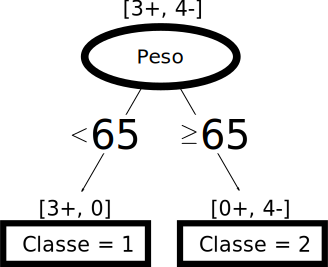
\includegraphics[width=0.4\textwidth]{imgs/slides2-tree.pdf}
\end{figure}


\section*{\textbf{Exercício folha}}
\addcontentsline{toc}{section}{Exercício folha}

% ----------------------------------------------------------
% Questão a
% ----------------------------------------------------------
\section*{\textbf{a) Qual o objetivo de se executar poda (\textit{prunning}) em árvores de decisão?}}
\addcontentsline{toc}{section}{a) Qual o objetivo de se executar poda (\textit{prunning}) em árvores de decisão?}

Existem dois objetivos principais, maximizar o desempenho da árvore de decisão em questão sem perder seu poder de decisão e reduzir seu tamanho físico, ou seja, tornar a árvore de decisão mais leve, irá ocupar menos espaço em disco. Um outro objetivo é evitar que os erros e ruídos presentes em ramificações muitos específicas da árvore atrapalhe na decisão tomada.

% ----------------------------------------------------------
% Questão b
% ----------------------------------------------------------
\section*{\textbf{b) Quais tipos de poda (\textit{prunning}) estão previstos na literatura?}}
\addcontentsline{toc}{section}{b) Quais tipos de poda (\textit{prunning}) estão previstos na literatura?}

Na literatura encontram-se diversos tipo de poda para árvore de decisão. Eles estão classificados em dois grandes grupos, os métodos \texttt{pré-poda} e \texttt{pós-poda}. Os métodos pré-poda são realizado durante a construção da árvore de decisão, ou seja, na sua construção um nodo pode parar de ser ramificado e transformado em nodo folha se os critérios para isto forem satisfeito. Já a pós-poda acontece após a construção completa da árvore, aonde a ramificação abaixo de um nodo é removida e este nodo passa a ser um nodo folha, representando a classe de maior representatividade na ramificação removida. Alguns métodos conhecidos que se destacam, são: \textit{Cost Complexity Pruning}, \textit{Reduced Error Pruning}, \textit{Minimum Error Pruning (MEP)}, \textit{Pessimistic Pruning}, \textit{ErrorBased Pruning (EBP)}, \textit{Minimum Description Length (MDL) Pruning}, \textit{Mininum Message Length (MML) Pruning}, \textit{Critical Value Pruning (CVP)}, \textit{OPT} e \textit{OPT-2}, conforme \citeonline{decision-tree-unicamp}.  

% ----------------------------------------------------------
% Questão c
% ----------------------------------------------------------
\section*{\textbf{c) Para o \textit{dataset} de exemplo, qual o impacto da poda (\textit{prunning}) nas árvores resultado? Quais são as diferenças perceptíveis entre as árvores geradas?}}
\addcontentsline{toc}{section}{c) Para o dataset de exemplo, qual o impacto da poda (prunning) nas árvores resultado? Quais são as diferenças perceptíveis entre as árvores geradas?}

O impacto gerado pela poda foi extremamente significativo, a árvore gerada com o algoritmo sem utilizar poda tinha um tamanho de 7976 nodos com 6812 nodos folha, após a utilização do algoritmo a árvore passou a ter um tamanho de 710 com 564 nodos folha, uma redução no tamanho da árvore e na quantidade de nodos folha de 91\%. A principal diferença percebida, é a ausência de ramificações existentes a partir de certos nodo, que é exatamente o que a poda realiza. Na \autoref{captura-tela}, podemos observar de maneira clara a poda que acontece no nodo \texttt{\textit{capital-gain $\le$ 3942}}.

\begin{figure}[H]
    \caption{Captura de tela}
    \label{captura-tela}
    \centering
    \includegraphics[width=\textwidth]{imgs/unpruned-vs-pruned.pdf}
\end{figure}


% Finaliza a parte no bookmark do PDF, para que se inicie o bookmark na raiz
% ---
\bookmarksetup{startatroot}% 
% ---

% ---
% Conclusão
% ---
% \section*{Considerações finais}
% \addcontentsline{toc}{section}{Considerações finais}

% ----------------------------------------------------------
% ELEMENTOS PÓS-TEXTUAIS
% ----------------------------------------------------------
\postextual

% ----------------------------------------------------------
% Referências bibliográficas
% ----------------------------------------------------------
\newpage
\nocite{material_aula}
\nocite{enunciado_aula}
\nocite{Witten:2016:DMF:3086818}
\bibliography{bibliography}

\end{document}